\documentclass[a4paper,14pt]{extarticle} % тип документа
\usepackage{extsizes}
\usepackage[left=3cm,right=2cm,top=2cm,bottom=2cm,bindingoffset=0cm,nohead]{geometry}
\usepackage{indentfirst}
\usepackage{cmap}
\usepackage[T2A]{fontenc}			% кодировка
\usepackage[utf8]{inputenc}			% кодировка исходного текста
\usepackage[english,russian]{babel}	% локализация и переносы
\usepackage{amsmath,amsfonts,amssymb,amsthm,mathtools,array} 
\usepackage{wasysym}
\usepackage[labelsep=period]{caption}
\usepackage{graphicx}
\usepackage{pgfplots}
\usepackage{makeidx}
\usepackage{tikz}
\usepackage{pgfplots}
\pgfplotsset{compat=1.18}
\usepackage{pdfpages}
\usepackage[nottoc,numbib]{tocbibind}
\usepackage{setspace}
\linespread{1.3}
\usepackage{nomencl}
\makenomenclature
\usepackage{totcount}
\usepackage{subcaption}
\usepackage{listings}
\usepackage{diagbox}
\usepackage{placeins}
% \renewcommand{\baselinestretch}{1.5} 
\regtotcounter{figure}
\regtotcounter{page}
\renewcommand{\nomname}{Сокращения и обозначения}
\newtotcounter{citnum}
\def\oldbibitem{} \let\oldbibitem=\bibitem
\def\bibitem{\stepcounter{citnum}\oldbibitem}
\newtotcounter{citesnum}
\def\oldcite{} \let\oldcite=\cite
\def\cite{\stepcounter{citesnum}\oldcite}

% \newcounter{mycitecount}                                %% Счётчик библиографии
% \AtEveryBibitem{\stepcounter{mycitecount}}              %% Работает для biblatex

% \usepackage[chaptercount,%
%             figure,      %
%             table,       %
%             apxcount,    %
%             basepage,    %
%             mycitecount, xspace ]{totalcount}           %% Подсчёт общего количества объектов в документе

\author{Кузнецов Игорь}
\title{}
\date{\today}

\renewcommand{\bottomfraction}{1.0} % часть страницы, которую может занимать графика снизу страницы

\newcolumntype{L}{>{$}l<{$}} % math-mode version of "l" column type
\newcommand{\ZE}{\bar{E}}
\newcommand{\BE}{\partial E}
\newcommand{\CE}{\complement E}
\newcommand{\IE}{\stackrel{\circ}{E}}
\newcommand{\Def}{\textbf{Определение }}
\newcommand{\Ter}{\textbf{Теорема }}
\newcommand{\Utv}{\textbf{Утверждение }}
\newcommand{\Prd}{\textbf{Предложение }}
\newcommand{\Dvo}{\textbf{Доказательство }}
\newcommand{\Imp}{\textbf{(!) }}
\newcommand{\Sld}{\textbf{Следствия: }}
\newcommand{\Svv}[1]{\textbf{Свойства #1:} }
\DeclareMathOperator{\Ree}{Re}
\DeclareMathOperator{\Imm}{Im}
\DeclareMathOperator{\res}{res}
\DeclareMathOperator{\cov}{cov\,}
\DeclareMathOperator{\kH}{\text{кН}}
\DeclareMathOperator{\m}{\text{м}}
\DeclareMathOperator{\kHm}{\kH\cdot\m}

\begin{document}
% \maketitle
\newcommand{\brv}[1]{{\left| #1 \right|}}
\newcommand{\brr}[1]{{\left( #1 \right)}}
\newcommand{\brs}[1]{{\left[ #1 \right]}}
\newcommand{\brc}[1]{{\left\{ #1 \right\}}}
\newcommand{\brn}[1]{{\left\lVert #1 \right\rVert}}
\newcommand{\bra}[1]{{\left\langle #1 \right\rangle}}
\newcommand{\brrl}[1]{{\left( #1 \right]}}
            \newcommand{\brrr}[1]{{\left[ #1 \right)}}
\newcommand{\under}[2]{{\underset{#2}{\underbrace{#1}}}}
\newcommand{\strm}[1]{\underset{#1}{\rightarrow}}
% 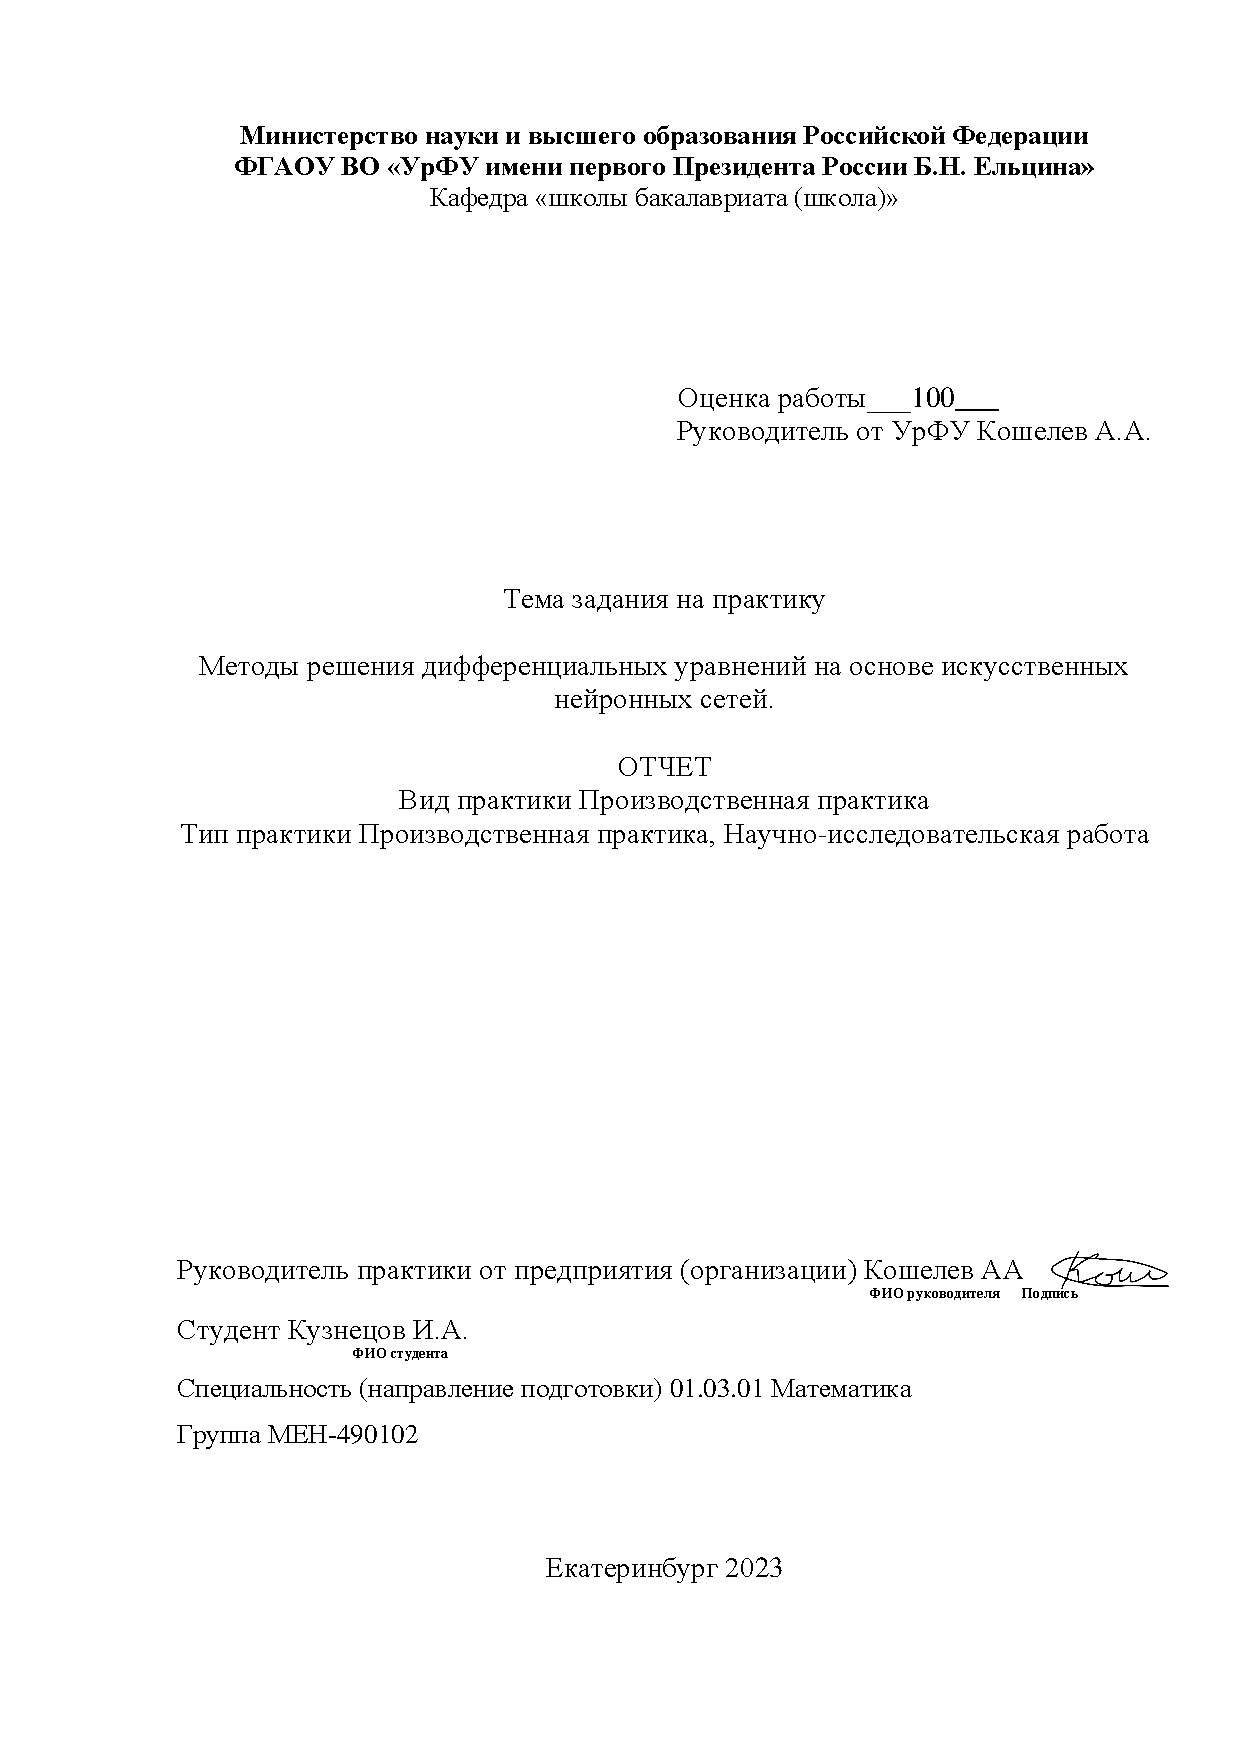
\includepdf{Отчет по практике (2).pdf}

% 

\begin{center}
    
    \section*{РЕФЕРАТ}
    \addcontentsline{toc}{section}{РЕФЕРАТ}
\end{center}

Кузнецов Игорь александрович <<Возможность использования искусственных нейронных сетей для решения задач математической физики>>:  работа содержит: страниц \total{page}, иллюстраций \total{figure}, использованных источников \total{citnum}

\noindent Ключевые слова: PINN, дифференциальные уравнения, электрокинетика, нейронные сети, python

% Целью работы является исследование возможности применения PINN (Physics-Informed Neural Networks) в решении задач 
PINN (Physics-Informed Neural Networks) - это метод, который сочетает в себе преимущества нейронных сетей и физических моделей для решения задач научного моделирования. В данном дипломном проекте исследуется применение метода PINN для решения задачи обратной задачи электрокинетики. В работе проводится анализ эффективности метода PINN в сравнении с классическими методами решения обратных задач. Также исследуется влияние различных параметров на точность рения задачи. Результаты исследования показывают, что метод PINN может быть эффективным инструментом для решения задач научного моделирования, особенно в случаях, когда классические методы неэффективны или недостаточно точны.
Были использованы следующие технологии:
\begin{itemize}
    \item язык программирования Python;
    \item библиотека для работы с глубокими нейронными сетями Tensorflow;
    \item библиотека ESPResSo, для проведения традиционных симуляций;
\end{itemize}
\newpage
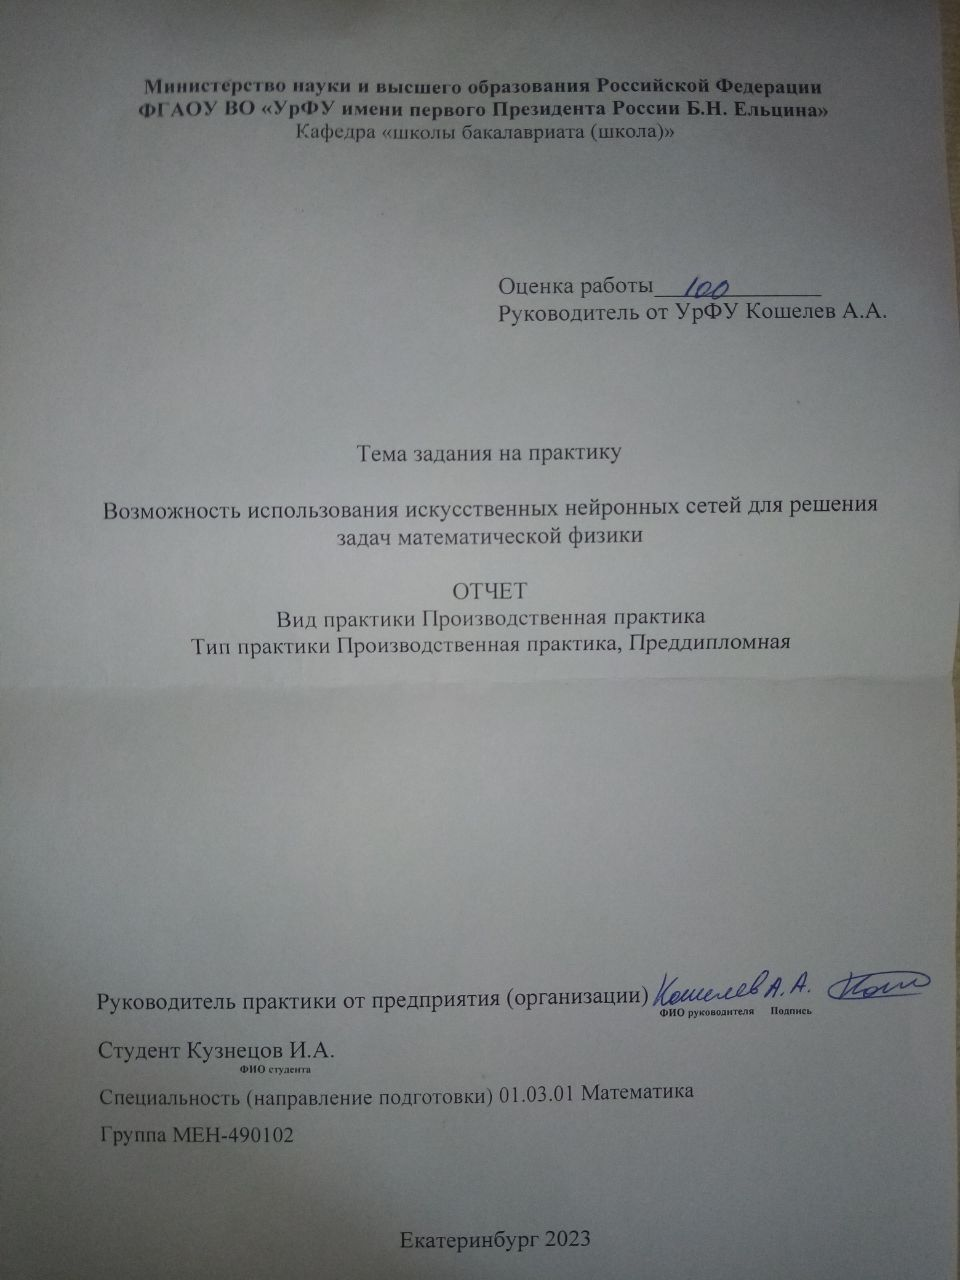
\includegraphics[width=\textwidth]{титульник.jpg}
\thispagestyle{empty}

\newpage
\tableofcontents
\newpage

% \section*{Обозначения и сокращения}

В настоящей работе применяют следующие обозначения и сокращения

\begin{description}
    \item[PINN] -- Physics-Informed neural network, физически информированная нейронная сеть
    \item[$c$] -- Концентрация ионных частиц
    \item[$j$] -- Поток плотности
    \item[$\vec{v}$] -- Адвективная скорость жидкости
    \item[$e$] -- Заряд электрона
    \item[$z$] -- Валентность частиц
    \item[$\Phi$] -- Электростатический потенциал
    \item[$\xi$] -- Подвижность частиц
    \item[$D$] -- Коэффициент диффузии частиц
    \item[$l_B$] -- Длина Бьеррума, $l_B = \frac{e^2}{4\pi\varepsilon k_B T}$
    \item[$k_B$] -- Постоянная Больцмана
    \item[$T$] -- Температура
    \item[$\rho$] -- Плотность жидкости
    \item[$p_H$] -- Гидродинамическое давление
\end{description}

% \noindent\begin{tabular}{llm{15cm}}
%     PINN & -- & Physics-Informed neural network, физически информированная нейронная сеть
% \end{tabular}

\newpage

% \\nomenclature \{(\$[a-z\\\{\}_]*\$)\}\{(.*)\}
% \\item[$1] -- $2
% \nomenclature {$c$}{Концентрация ионных частиц}
% \nomenclature {$j$}{Поток плотности}
% \nomenclature {$\vec{v}$}{Адвективная скорость жидкости}
% \nomenclature {$e$}{Заряд электрона}
% \nomenclature {$z$}{Валентность частиц}
% \nomenclature {$\Phi$}{Электростатический потенциал}
% \nomenclature {$\xi$}{Подвижность частиц}
% \nomenclature {$D$}{Коэффициент диффузии частиц}
% \nomenclature {$l_B$}{Длина Бьеррума, $l_B = \frac{e^2}{4\pi\varepsilon k_B T}$}
% \nomenclature {$k_B$}{Постоянная Больцмана}
% \nomenclature {$T$}{Температура}
% \nomenclature {$\rho$}{Плотность жидкости}
% \nomenclature {$p_H$}{Гидродинамическое давление}

% \printnomenclature


\section{Введение}

В последние годы нейронные сети получили широкое распространение, они широко используются для анализа и генерации изображений и видео, обработки естественных языков (перевод, чат-боты), медицинской диагностике, финансовых прогнозах и так далее.

Одним из перспективных направлений в этой области являются так называемые PINN -- Physics-Informed Neural Networks, физически-инфор\-мированные нейронные сети. Классические нейронные сети используют большую выборку реальных данных, однако в естественно-научных областях, таких как физика, химия, биология и т.д. зачастую может просто не хватать нужного объёма данных для обучения. PINN способны обойти это ограничения, используя в обучении знания законов физики, описываемые дифференциальными уравнениями в частных производных. Это позволяет использовать неполные и зашумленные данные, что делает их полезными в реальных научных задачах. Однако, вычислительная сложность PINN выше, чем у классических нейронных сетей, что требует большого количества вычислительных мощностей.

Впервые терми PINN был введён в статье \cite{bib:pinn:first}. В ней автор дал формальное определение PINN'ам и рассмотрел решение нескольких задач: уравнение Шрёдингера, Навье-Стокса, Ален-Чана.

В настоящее время PINN широко применяются моделировании, анализе широкого спектра физических явлений:

В статье \cite{bib:voltogr:1} рассматривается задача симуляции циклической вольтаметрии, исследователями было рассмотрено несколько случая: одномерная вольтаметрия на дисковом электроде с полубесконечными или тонкослойными граничными условиями, двумерная вольтаметрия на микрополосковом электроде и наконец вольтаметрия на края квадратного электрода, количественно определяя неравномерное распределение тока вблизи угла электрода. Для моделирования был использован перцептрон использующий от трёх до шести скрытых слоёв, и гиперболический тангенс в качестве функции активации. Полученные исследователями данные хорошо согласуются с решениями этих же задач, полученными другими способами.

Так же PINN применяются для: анализа литий-ионных батарей\cite{bib:lbat:1,bib:lbat:2}, для моделирование теплопереноса в системах со сложной геометрией \cite{bib:heat:1,bib:heat:2}, решения уравнения Навье-Стокса для моделирования турбулентности \cite{bib:navstock:1}, химической кинематике \cite{bib:chemkin:1,bib:chemkin:2}. Для изучения биологических процессов существует разновидность PINN'ов -- BINN (Biologically-informed neural network) \cite{bib:BINN:1}

\newpage
\section{Постановка задачи}

\subsection{Цель работы}

% Рассмотреть уже решённую физическую задачу, решить её с помощью PINN и сравнить полученные данные с изначальным решением, оценить целесообразность применения PINN к задаче.

Рассмотреть задачу распределения тепла в диске, решить её с помощью PINN и сравнить полученные данные с изначальным решением, оценить целесообразность применения PINN к задаче.

\subsection{Описание задачи}

Создать нейросеть, которой на вход подаются пространственные координаты. На выходе хотим получить температуру в данной точке. Обучить данную нейросеть используя PINN. Провести оценку результатов обучения: скорости, точности ответа.

\newpage
\section{Теоретическое описание PINN}

Пусть система описывается некой системой дифференциальных уравнений:
\begin{equation}\label{eq:1syst}
    F_j(t, x, u, \lambda_j) = 0, x\in\Omega, t > 0, j=\overline{1,N}
\end{equation}
с граничными условиями
\begin{equation}
    B_k(t_0,x_0, u) = 0, t_0, x_0 \in \text{граничные точки}
\end{equation}
где $t$ -- время, $x$ -- пространственные координаты, $\Omega$ -- некоторая область в пространстве $\mathbb{R}^n$,  $u(t,x)$ -- искомая функция описывающая интересующие нас свойства системы (скорость, концентрация, потенциал и т.п.), $\lambda_j$ -- векторы постоянных параметров системы, такие как плотность вещества, заряд частиц, теплопроводность материала, температура окружающей среды и тому подобное.

Определим $f(t, x)$ следующим образом:

\begin{equation}
    f(t, x):=\begin{pmatrix}
        F_1(t,x,u) \\
        F_2(t,x,u) \\
        \dots      \\
        F_N(t,x,u)
    \end{pmatrix}
\end{equation}

где $u(t,x)$ аппроксимируется с помощью глубокой нейронной сети. $f(t,x)$ назовём физически-информированной нейросетью, или же PINN, она может быть получена с помощью автоматического дифференцирования сложных функций. Данная имеет все те же параметры, что и сеть $u(t,x)$, а так же дополнительно набором параметров $\lambda$.

Для обучения нейросети составим следующую функцию потерь:

\begin{equation}
    MSE = MSE_f + MSE_u
\end{equation}
где
\begin{equation}
    MSE_f = \sum_{j=1}^N\frac{1}{N_f}\sum_{i=1}^{N_f} F_j^2(t^i_f, x^i_f, u(t^i_f, x^i_f))
\end{equation}
требует соблюдения дифференциальных уравнений, описывающих процесс, здесь $\brc{t^i_f, x^i_f}_{i=1}^{N_f}$ -- точки коллокации для $F_j$, $N_f$ -- количеств этих точек и
\begin{equation}
    MSE_u = \frac{1}{N_u}\sum_{i=1}^{N_u} ((u(t^i_u, x^i_u)) - u^i_0)^2
\end{equation}
требует соблюдения граничных условий $\brr{t^i_0, x^i_0, u^i_0}_{i=1}^{N_0}$ для функции $u(t,x)$. Принципиальная схема работы PINN изображена на рисунке~\ref{fig:pinn_scheme}

\begin{figure}[ht]
    \center
    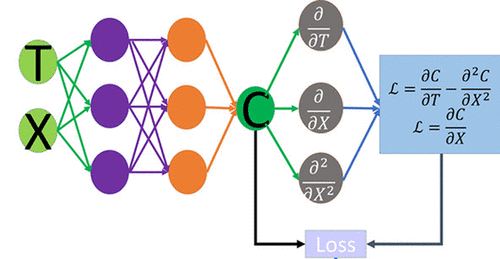
\includegraphics{PINN scheme.png}
    \caption{Принципиальная схема работы PINN}
    \label{fig:pinn_scheme}
\end{figure}

\FloatBarrier
\newpage
\section{Техническая реализация}
\subsection{Используемые технологии}

% В данном разделе обсудим технологии, необходимые для создания PINN

Для разработки будем использовать язык Python 3.10.6 -- высокоуровневый язык программирования общего назначения, один из наиболее популярных языков в области машинного обучения и Tensorflow -- библиотеку для создания и обучения нейронных сетей. Выбор данной библиотеки обусловлен простотой создания нейронных сетей, высокой производительностью, а так же встроенным автоматическим дифференцированием, которое и позволит нам обучить нейросеть дифференциальным уравнениям в частных производных.

\subsection{Общая архитектура PINN}

В качестве архитектуры нейронной сети, аппроксимирующей функцию $u(t,x)$ возьмём многослойный перцептрон, точное число слоёв и нейронов в каждом слое будем выбирать экспериментально, в качестве функции активации слоя будем использовать $\tanh$. Для создания нейронной сети воспользуемся классом \texttt{tensorflow.keras.Model}, для создания слоёв классом \texttt{tensorflow.keras.layers.Dense}. PINN $f(t, x)$ будет иметь всего один слой. Параметрами этого слоя и есть параметры $\lambda_j$ из системы (\ref{eq:1syst}). На вход слой получает $N_f$ точек (\ref{eq:1syst}) и $N_u$ точек для граничных условий. Внутри этого слоя мы считаем частные производные $u(t,x)$ с помощью \texttt{tensorflow.GradientTape}, и составлять из них и параметров $\lambda_j$ систему уравнений (\ref{eq:1syst}). На выход из данного слоя будем выдавать значения $u(t,x)$ и сами эти уравнения. В силу вида системы (\ref{eq:1syst}) все выходы, соответствующие уравнениям системы (\ref{eq:1syst}) должны быть равны 0. В качестве оптимизатора будем использовать Adam, а в качестве метрики MSE

% \setstretch{1.0}
% \begin{lstlisting}[language=Python]
% def build_net(layers, activation, dim, **kwargs):
%     ins = tf.keras.layers.Input(shape=(1+dim,))
%     x = ins
%     for layer in layers:
%         x = tf.keras.layers.Dense(layer, activation=activation,
%                                   kernel_initializer='he_normal')(x)

%     outs = {
%         "c": tf.keras.layers.Dense(1, kernel_initializer='he_normal')(x),
%         "Fi": tf.keras.layers.Dense(1, kernel_initializer='he_normal')(x),
%     }
%     return tf.keras.models.Model(inputs=ins, outputs=outs)
% \end{lstlisting}
% \setstretch{1.5}

\FloatBarrier
\newpage
\section{Эксперименты}

\subsection{Установившееся распределение тепла в кольце}

Рассмотрим для начала относительно простую задачу: определить распространение тепла, установившееся в кольце $1<r<2.\; 0<\phi<2\pi$, с граничными условиями:
\begin{equation}
    \begin{aligned}
        u(1,\phi)=&\cos\phi+\sin\phi+\sin(2\phi)+5\sin(3\phi)+1\\
        u(2,\phi)=&\sin(2\phi)+\sin(3\phi)+\cos(4\phi)
    \end{aligned}
\end{equation}
Установившееся распространение тепла описывается уравнением Пуассона, учитывая что внутренних источников тепла нет получаем:
\begin{equation}
    \Delta u = 0
\end{equation}

Для полярных координат оно принимает вид

\begin{equation}
    \frac{\partial^2 u}{\partial r} + \frac{1}{r} \frac{\partial u}{\partial r} + \frac{1}{r^2}\frac{\partial^2 u}{\partial \phi^2} = 0
\end{equation}

Данная задача имеет аналитическое решение:

\begin{equation}\label{eq:termal}
    \begin{split}
        u(r,\phi) & = 1-\frac{\ln r}{\ln 2}\\
        &+\brr{\frac{-r}{3}+\frac{4}{3r}}\sin(\phi)+\brr{\frac{-r}{3}+\frac{4}{3r}}\cos(\phi)\\
        &+\brr{\frac{r^2}{5}+\frac{4}{5r^2}}\sin(2\phi)\\
        &+\brr{\frac{3r^3}{63}+\frac{312}{64r^3}}\sin(3\phi)\\
        &+\brr{\frac{16r^4}{255}-\frac{16}{255r^4}}\cos(4\phi)
    \end{split}
\end{equation}

% Запустим обучение со следующими конфигурациями скрытых слоёв:
% \begin{itemize}
%     \item 20, 20, 20
%     \item 50, 50, 50
% \end{itemize}

% Для одной итерации обучения возьмём по одной точке для каждого граничного условия \ref{eq:termal_cond} и одну внутреннюю точку для уравнения (\ref{eq:termal}), всего 3 точки на итерацию, точки выбираются случайным образом. Рассмотри случаи с 1000, 10000 и 100000 точек. Обучать будем в течении 1000 эпох или пока ошибка не будет улучшаться в течении 10 эпох хотя бы на 0.0001, размер батча 32. График обучения изображён на рисунке~\ref{fig:termal_loss}, время обучения указано в таблице \ref{table:termal_time}

% Для одной итерации обучения возьмём по одной точке для каждого граничного условия \ref{eq:termal_cond} и одну внутреннюю точку для уравнения (\ref{eq:termal}), всего 3 точки на итерацию, точки выбираются случайным образом. Рассмотри случаи с количеством точек $N = 1000, 10000, 100000$. В каждом случае обучать будем в течении $10000000/N$, таким образом число итераций во всех случаях будет одинаково и можно будет оценить зависимость скорости обучения и итоговой точности от числа точек. Так же для сокращения времени обучения будем прерывать его, если в течении 1000 эпох не происходит улучшение функции потерь хотя бы на 0.0001. Размер батча 32 -- стандартный размер батча в \texttt{tensorflow}. График обучения изображён на рисунке~\ref{fig:termal_loss}, время обучения указано в таблице \ref{table:termal_time}

Для одной итерации обучения возьмём $N_f$ внутренних точек для уравнения (\ref{eq:termal}) и $N_u$ точек для внутреннего и внешнего условий, обозначим их количество как $N_i$ и $N_o$ соответственно, всего $N_f+2N_u$ точек. В данном случае функция потерь будем выглядеть следующим образом:

\begin{equation}\label{eq:termal_cond}
    \begin{split}
        MSE =& \frac{1}{N_f}\sum_{i=1}^{N_f} \brr{ \frac{\partial^2 u}{\partial r}(r_i, \phi_i) + \frac{1}{r} \frac{\partial u}{\partial r}(r_i, \phi_i) + \frac{1}{r^2}\frac{\partial^2 u}{\partial \phi^2}(r_i, \phi_i)}^2 + \\
        & \frac{1}{N_i}\sum_{i=1}^{N_i} \brr{u(1, \phi_i) - \cos\phi+\sin\phi+\sin(2\phi_i+5\sin(3\phi_i+1}^2 + \\
        & \frac{1}{N_o}\sum_{i=1}^{N_o} \brr{u(2, \phi_i) - \sin(2\phi_i+\sin(3\phi_i+\cos(4\phi_i}^2
    \end{split}
\end{equation}

Возьмём сеть со скрытыми слоями [20,20,20,20] и проведём вычисления при различных значениях для $N_f$ и $N_u$. Эпох 10000, размер батча 32 -- стандартный размер батча в \texttt{tensorflow}. Валидацию буем следующим образом: для уравнения~(\ref{eq:termal}) разобьём область на радиальную сетку, с числом узлов $N_f$ и сторонами $dr, d\phi$, так что бы $dr~d\phi$, для граничных условий~(\ref{eq:termal_cond}) равномерно расположим на $[0, 2\pi]$ $N_u$ точек.

По графикам обучения, изображённым на рисунке~\ref{fig:termal_loss} видно, что при малом количестве внутренних точек $N_f$ значения функции потерь на валидационной выборке в несколько раз больше значений функции потерь на обучающей выборке, с увеличением $N_f$ же значения функции потерь на обучающей и валидационной выборках практически совпадаю.

\begin{figure}[htb!]
    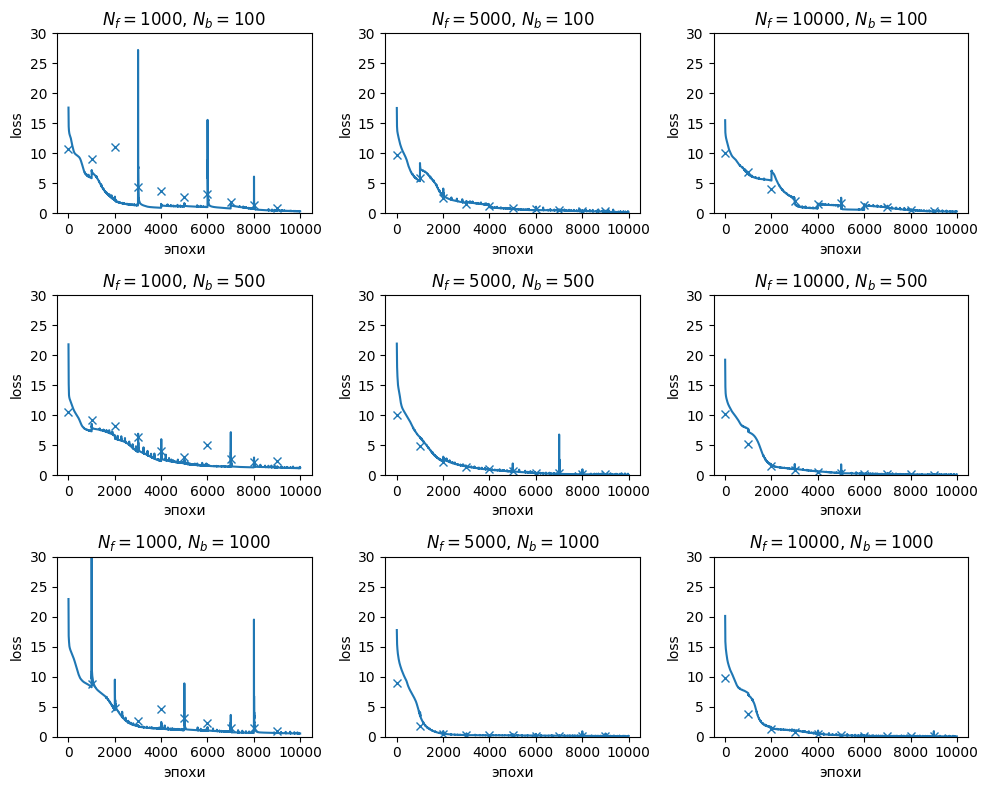
\includegraphics[width=\textwidth]{../plots/termal/loss l = (20x4) Nf=[1000, 5000, 10000] Nu=[100, 500, 1000].png}
    \caption{Графики функций потерь для различных сочетаний $N_f$ и $N_u$, крестиками изображаются результаты валидации в определённые моменты времени}
    \label{fig:termal_loss}
\end{figure}

% \begin{table}[htb]
%     \center
%     \begin{tabular}{|c|c|c|c|}
%         \hline
%         \diagbox{$N_f$}{$N_u$} & 1000 & 5000 & 10000\\
%         \hline
%         1000 & 10.06 & 85.62 & 401.14\\ 
%         \hline
%         50000 & 12.68 & 51.69 & 173.97\\
%         \hline
%         100000 & 12.68 & 51.69 & 173.97\\
%         \hline
%     \end{tabular}
%     \caption{Лучшее значение валидации для различных сочетаний $N_f$ и $N_u$}
%     \label{table:termal_loss}
% \end{table}

% \begin{table}[htb]
%     \center
%     \begin{tabular}{|c|c|c|c|}
%         \hline
%         \diagbox{Слои}{Итераций} & 1000 & 10000 & 100000\\
%         \hline
%         [20, 20, 20] & 10.06 & 85.62 & 401.14\\
%         \hline
%         [50, 50, 50] & 12.68 & 51.69 & 173.97\\
%         \hline
%     \end{tabular}
%     \caption{Время обучения в секундах}
%     \label{table:termal_time}
% \end{table}

Время обучения, указанное в таблице \ref{table:termal_time} практически не зависит от количества точек для граничных условий $N_u$, вероятно потому что с ними не производится вычисление производных, а так же потому что их в целом меньше. В целом время обучения получается достаточно большим, возможным решением данной проблемы может быть изменение числа слоёв и количества нейронов в слоях.

\begin{table}[htb]
    \center
    \begin{tabular}{|c|c|c|c|}
        \hline
        \diagbox{$N_u$}{$N_f$} & 1000 & 5000 & 10000\\
        \hline
        100 & 311.65 & 1108.51 & 3494.39\\ 
        \hline
        500 & 314.31 & 1112.09 & 3487.54\\
        \hline
        1000 & 312.27 & 1109.55& 3472.66\\
        \hline
    \end{tabular}
    \caption{Время обучения в секундах для различных сочетаний $N_f$ и $N_u$}
    \label{table:termal_time}
\end{table}

Выполнение граничных условий при различных $N_u$ изображено на рисунках \ref{fig:termal_bnd1},\ref{fig:termal_bnd2},\ref{fig:termal_bnd3}. Для всех случаев характерно то, что внутренне условие при $r=1$ выполняется почти идеально, исключение составляет случай $N_f=1000, N_u = 500$, у которого изгибается конец, связанно это вероятно со стохастической природой оптимизатора Adam. Внешнее условие однако выполняется относительно плохо. Связанно такое различие вероятнее всего с тем, что разброс величин у внутреннего условия больше -- от -4 до 8, в то время как у внешнего в два раза меньше от -3 до 2, для решения данной проблемы в дальнейшем можно попробовать внести весовой коэффициент для граничного условия равный $\frac{1}{\max_\phi{u(r_0, \phi)}}$.

% \begin{figure}
%     \begin{subfigure}[b]{0.32\textwidth}
%         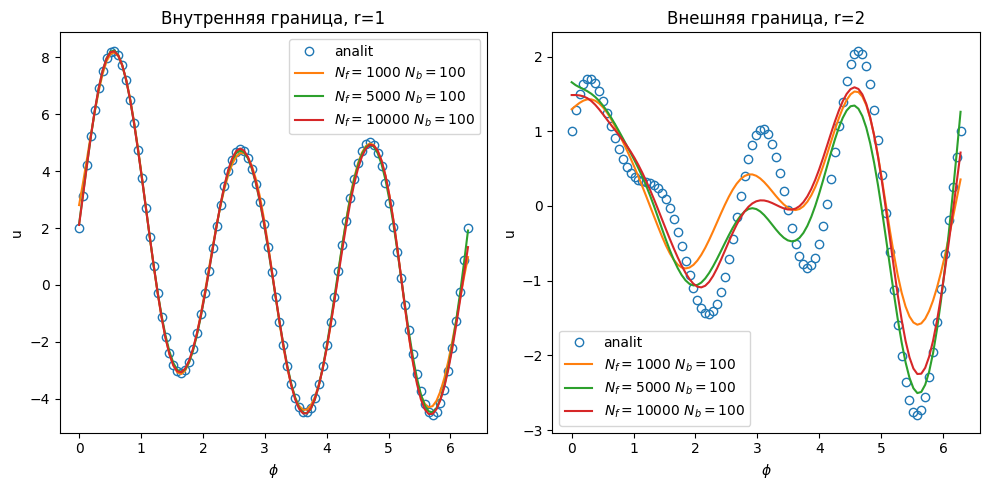
\includegraphics[width=\textwidth]{../plots/termal/bnd l = (20x4) Nf=[1000, 5000, 10000] Nu=100.png}
%     \end{subfigure}
%     \hfil
%     \begin{subfigure}[b]{0.32\textwidth}
%         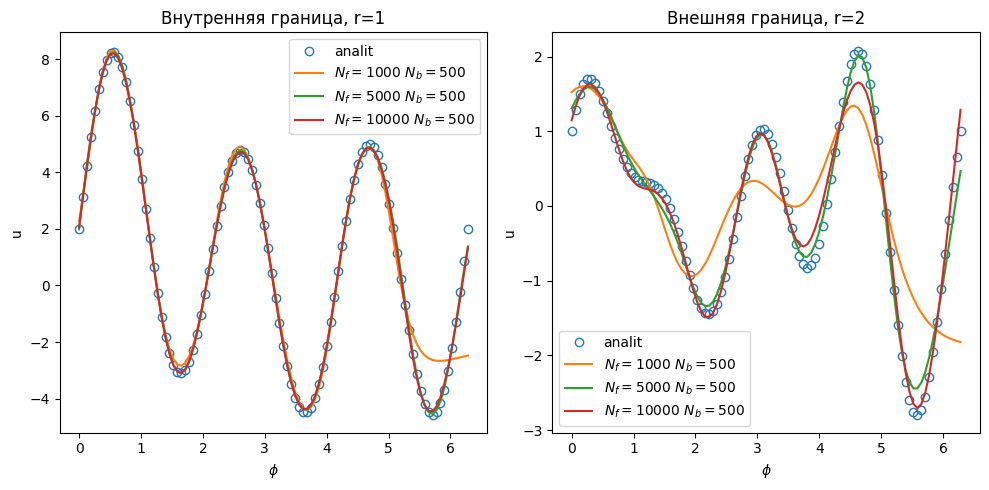
\includegraphics[width=\textwidth]{../plots/termal/bnd l = (20x4) Nf=[1000, 5000, 10000] Nu=500.png}
%     \end{subfigure}
%     \hfill
%     \begin{subfigure}[b]{0.32\textwidth}
%         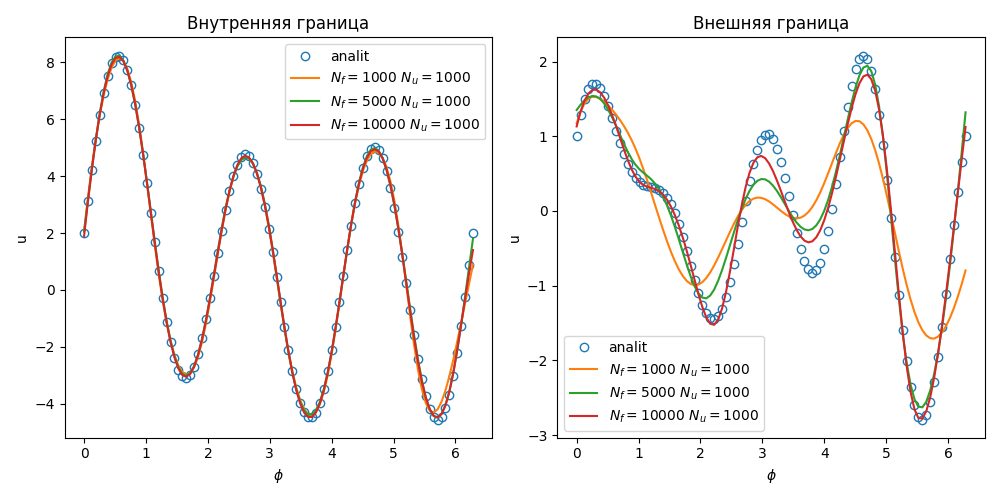
\includegraphics[width=\textwidth]{../plots/termal/bnd l = (20x4) Nf=[1000, 5000, 10000] Nu=1000.png}
%     \end{subfigure}
% \end{figure}

\begin{figure}[ht]
    \center
    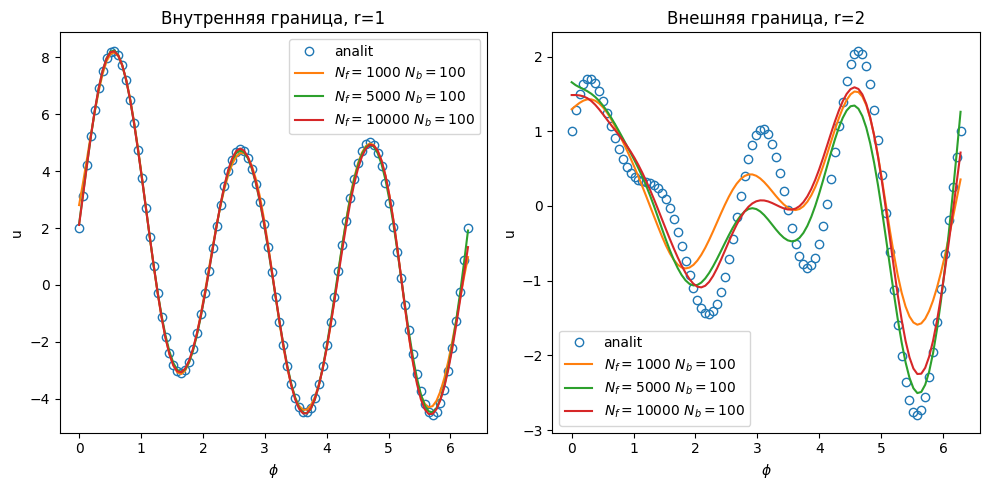
\includegraphics[width=0.7\textwidth]{../plots/termal/bnd l = (20x4) Nf=[1000, 5000, 10000] Nu=100.png}
    \caption{Граничные условия для случая $N_u=100$}
    \label{fig:termal_bnd1}
\end{figure}
\begin{figure}[ht]
    \center
    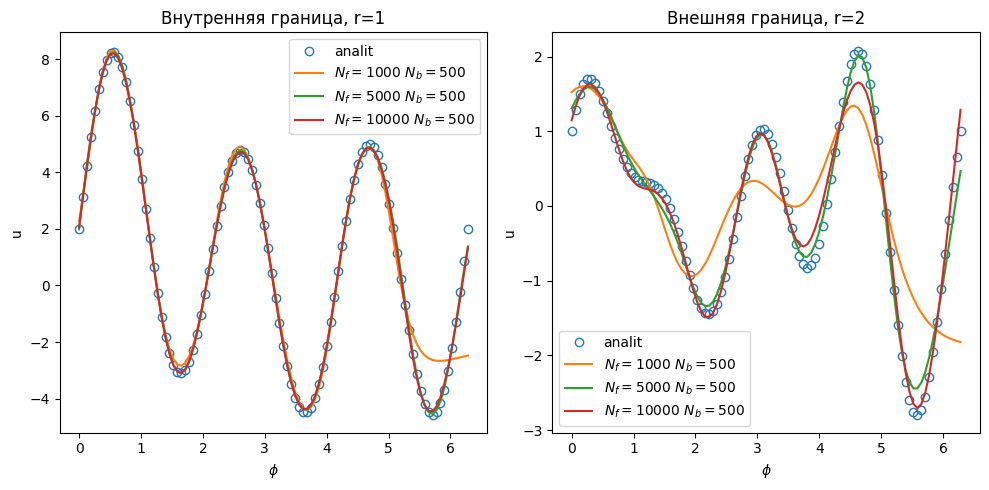
\includegraphics[width=0.7\textwidth]{../plots/termal/bnd l = (20x4) Nf=[1000, 5000, 10000] Nu=500.png}
    \caption{Граничные условия для случая $N_u=500$}
    \label{fig:termal_bnd2}
\end{figure}
\begin{figure}[ht]
    \center
    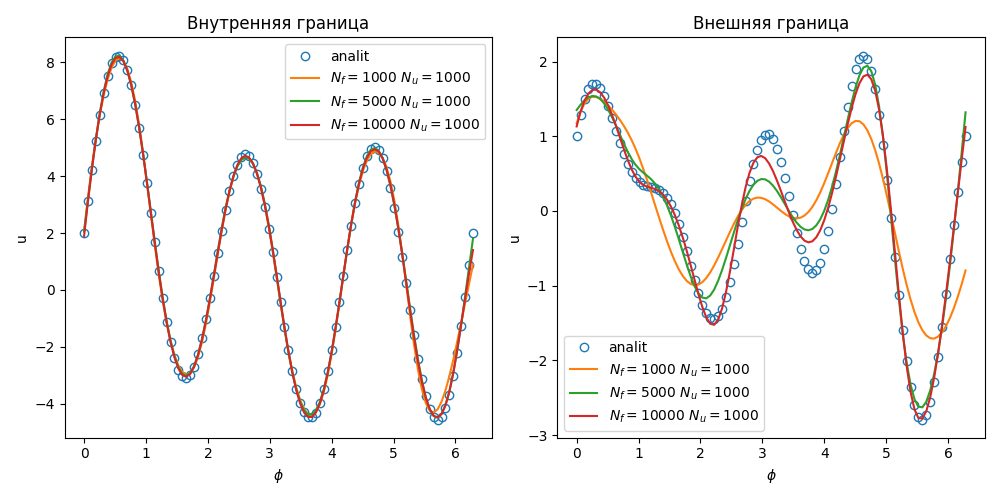
\includegraphics[width=0.7\textwidth]{../plots/termal/bnd l = (20x4) Nf=[1000, 5000, 10000] Nu=1000.png}
    \caption{Граничные условия для случая $N_u=1000$}
    \label{fig:termal_bnd3}
\end{figure}
\FloatBarrier

% Как видно из графика~\ref{fig:termal_loss} число нейронов в слое не оказывает существенного влияния на сходимость и точность сети, в то время как количество точек оказывает.

% Точки для обучения возьмём по $N$ точке для граничных условий и ещё $N$ точек для внутренних, всего $3N$ точек, где $N = 1000, 10000, 10000$. Обучать будем в течении 1000 эпох или пока ошибка не будет улучшаться в течении 10 эпох хотя бы на 0.001, размер батча.

% \subsection{Задача электрокинетики}

Для примера возьмём систему из \cite{bib:tutor}. Она описывается следующими уравнениями
$$\begin{aligned}
        \vec{j}                                                               & =
        -D \nabla c - \xi z e c \nabla \Phi + c \vec{u}                                    \\
        \partial_{t} c                                                        & =
        -\nabla \cdot\vec{j}                                                               \\
        \nabla^2 \Phi                                                         & =
        -4 \pi l_\mathrm{B} k_\mathrm{B}T z c                                              \\
        \rho \big( \partial_t \vec{u} + (\vec{u} \cdot \nabla ) \vec{u} \big) & =
        -\nabla p_H + \eta \nabla^{2} \vec{u} - (k_\mathrm{B}T \nabla c + zec \nabla \Phi) \\
        \nabla \cdot \vec{u}                                                  & =
        0
    \end{aligned}$$

Здесь первое уравнение в системе описывает поток плотности, второе электростатику, третье гидродинамику с помощью уравнения Навье-Стокса, четвёртое уравнение несжимаемости жидкости.

Рассмотрим систему щелевых пор, состоящую из двух одноимённо заряженных бесконечных пластин. Выпишем для такой системы граничные условия

$$
    \begin{aligned}
        c(t, X_l)       & = 0.01        \\
        c(t, X_r)       & = 0.01        \\
        c(0, X)         & = 0.002       \\
        \vec{v}(t, X_l) & = 0           \\
        \vec{v}(t, X_r) & = 0           \\
        \vec{v}(0, X)   & = 0           \\
        \Phi(t, X_l)    & = -0.05       \\
        \Phi(t, X_r)    & = -0.05       \\
        \Phi(0, X)      & = -0.009x^2+2
    \end{aligned}
$$
здесь $t$ -- время, $X_l$ -- пространственные координаты, соответствующие левой стенке, $X_r$ -- правой, $x$ в формул для $\Phi(0,x)$ соответствует оси, перпендикулярной пластинам.

\subsection{Упрощённый случай}

В начале рассмотрим упрощённую систему уравнений с одной пространственной координатой и без скорости

$$
    \begin{aligned}
        \frac{dc}{dT} & = -\nabla \cdot (- D\nabla c - \xi z e c \nabla \Phi) \\
        \nabla^2 \Phi & = -4 \pi l_\mathrm{B} k_\mathrm{B}T c
    \end{aligned}
$$

С граничными условиями

$$
    \begin{aligned}
        \frac{dc}{dX}(t, 0) & = 0 \\
        \frac{dc}{dX}(t, 1) & = 0 \\
        c(0, X)             & = 1 \\
        \Phi(0)             & = 1 \\
        \Phi(1)             & = 1 \\
    \end{aligned}
$$

Координаты в данном случае нормализованны

$$T = t/t_{\max},\;  X = (x+x_{\min})/x_{\max}$$

где $t_max$ -- время симуляции, $x_max$ -- размер системы по $x$-овой координате, $x_{\min}$ - координата левой стенки. Оператор $\nabla$ действует по пространственным координатам $\nabla = (\frac{d}{d X})$, все константы положим равными 1 и исключим $4\pi$ из второго уравнения.

Запустим обучение следующим образом: 100 запусков обучения (функция \texttt{fit}) по 10 эпох на 10000 наборах точек (внутренняя, граничная и начальная). Обучение заняло 2 минуты 48 секунд, значение функции потерь: $1.7378\cdot 10^{-5}$. Результаты симуляции представлены на рис.~\ref{fig:1d:simp:c} \ref{fig:1d:simp:Fi}:

\begin{figure}[ht]
    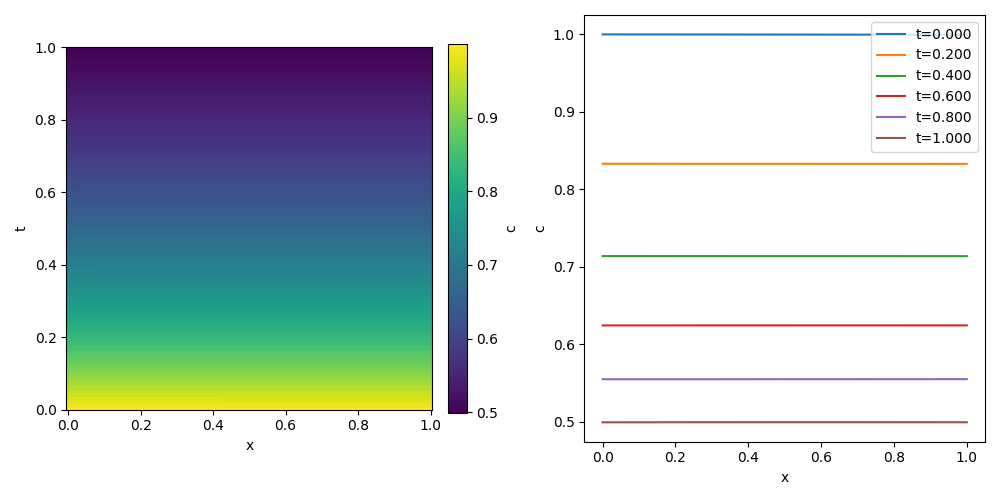
\includegraphics[width=\textwidth]{../plots/1-dim c simpified tanh 80,20.png}
    \caption{Упрощённый случай: концентрация}
    \label{fig:1d:simp:c}
\end{figure}

\begin{figure}[ht]
    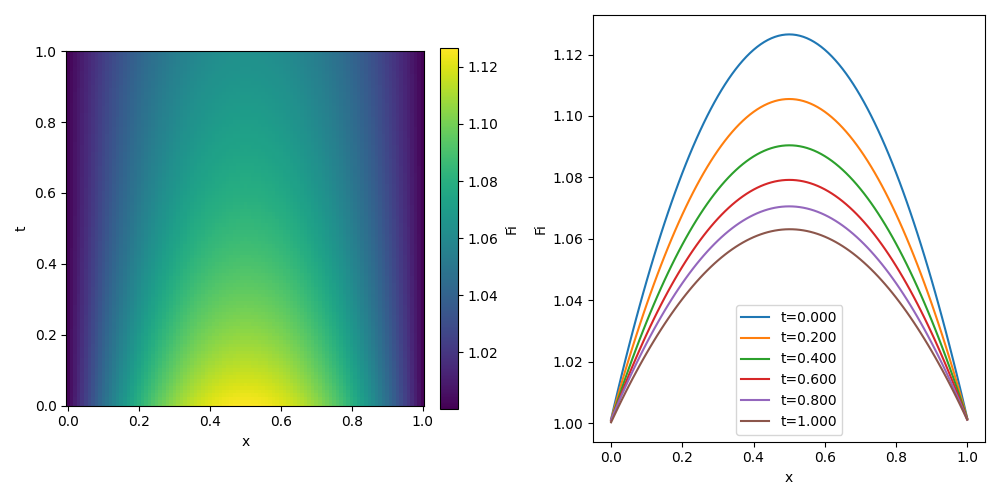
\includegraphics[width=\textwidth]{../plots/1-dim Phi simpified tanh 80,20.png}
    \caption{Упрощённый случай: потенциал}
    \label{fig:1d:simp:Fi}
\end{figure}

\subsection{Полный случай}

Рассмотрим двумерный случай. Скрытые слои будут иметь размеры 80 и 40, входной слой 4, один для концентрации, два для скорости и один для потенциала, функция активации $\tanh$ (гиперболический тангенс). Результат работы после 5000000 итераций показан на графике \ref{fig:2dres}

\begin{figure}[ht]
    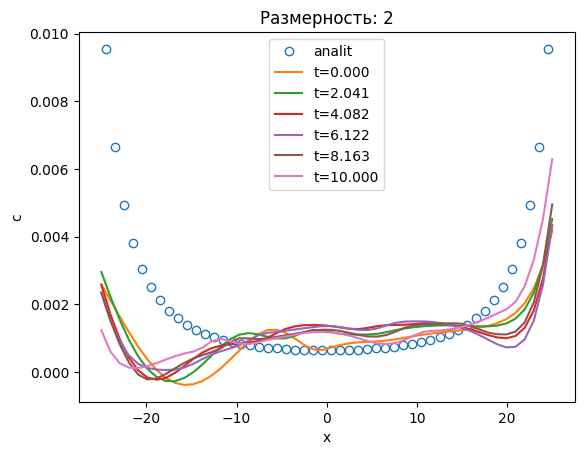
\includegraphics[scale=0.5]{../plots/2dim tanh 80 20.png}
    \caption{}
    \label{fig:2dres}
\end{figure}

Рассмотрим теперь трёхмерный случай. Скрытые слои так же будут иметь размеры 80 и 40, входной слой 5, один для концентрации, три для скорости и один для потенциала, функция активации $relu$. Результат работы после 30000000 итераций показан на графике \ref{fig:3dres}

\begin{figure}[ht]
    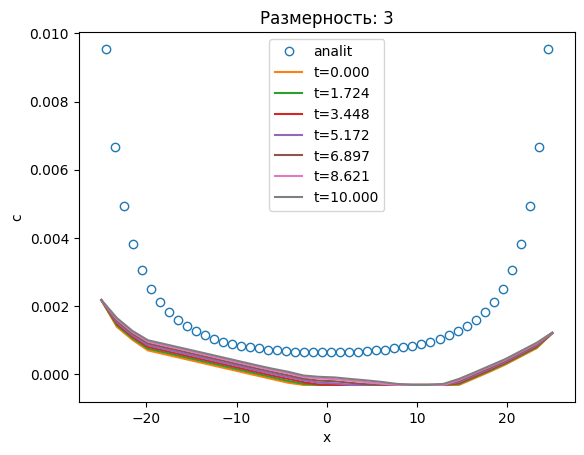
\includegraphics[scale=0.5]{../plots/3dim relu 80 20 30000000.png}
    \caption{}
    \label{fig:3dres}
\end{figure}

Наконец посмотрим на решение в целом. Точное решение изображено на графике~\ref{fig:termal_analit}, решение при различных $N_f$ и $N_u$ изображено на графике~\ref{fig:termal_pred}, ошибка между аналитическим решением и предсказаниями нейросети на графике~\ref{fig:termal_dif}. В целом графики достаточно хорошо совпадают в области. Расхождения наблюдаются в основном на стыке, где $\phi=0$. Что бы решить данную проблему можно попробовать добавить условие равенства $u(r, 0) = u(r, \phi)$, такому условию будет соответствовать следующая функция потерь:

\begin{equation}
    MSE_s = \frac{1}{N_s}\sum_{i=1}^{N_s} (u(r_i, 0) - u(r_i, 2\pi))^2
\end{equation}

Здесь $\brr{r_i}_{i=0}^{N_s}$ -- точки для данного условия, $N_s$ -- их количество.

\begin{figure}[ht]
    \center
    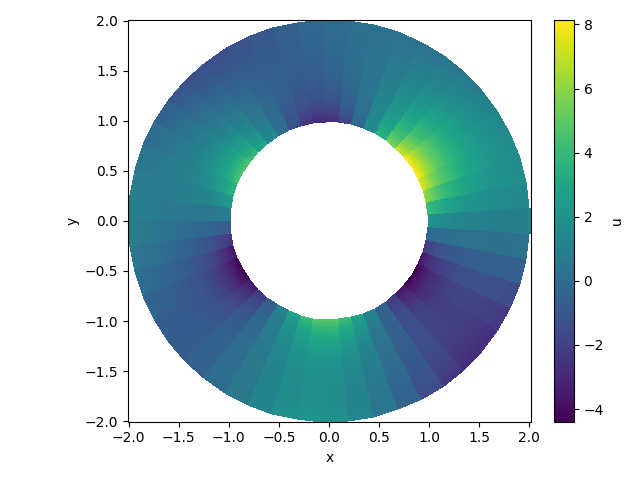
\includegraphics[width=0.5\textwidth]{../plots/termal/solut analit.png}
    \caption{Аналитическое решение}
    \label{fig:termal_analit}
\end{figure}

\begin{figure}[ht]
    \center
    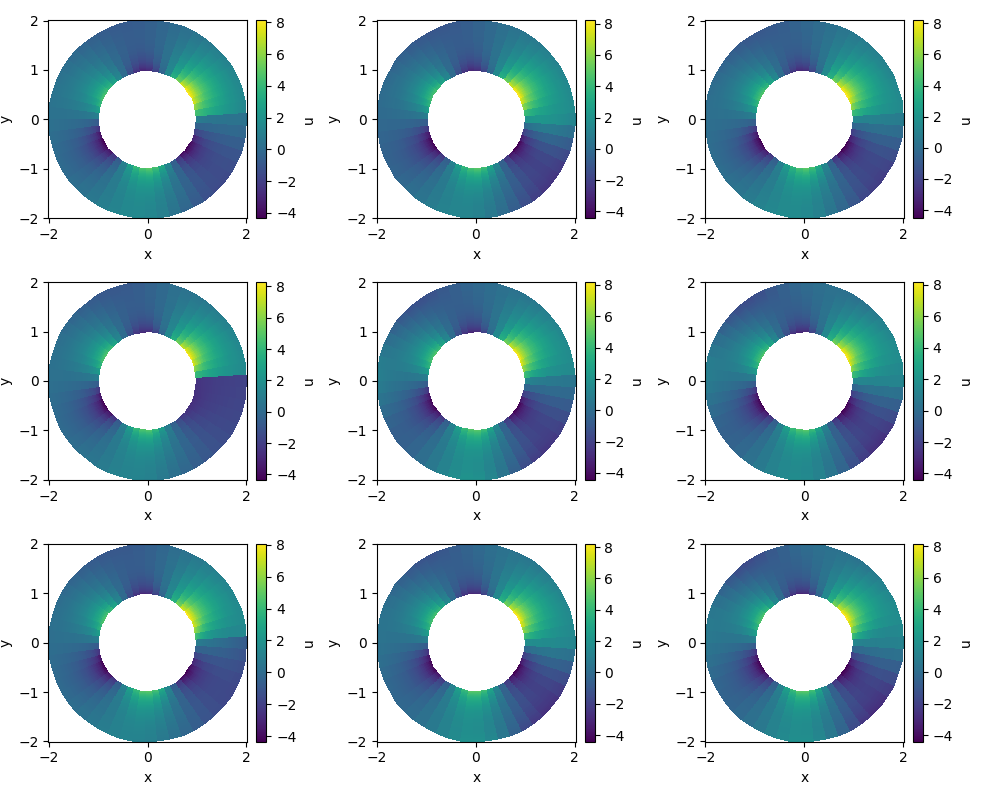
\includegraphics[width=\textwidth]{../plots/termal/solut l = (20x4) Nf=[1000, 5000, 10000] Nu=[100, 500, 1000].png}
    \caption{Решение при различных $N_f$ и $N_u$}
    \label{fig:termal_pred}
\end{figure}

\begin{figure}[ht]
    \center
    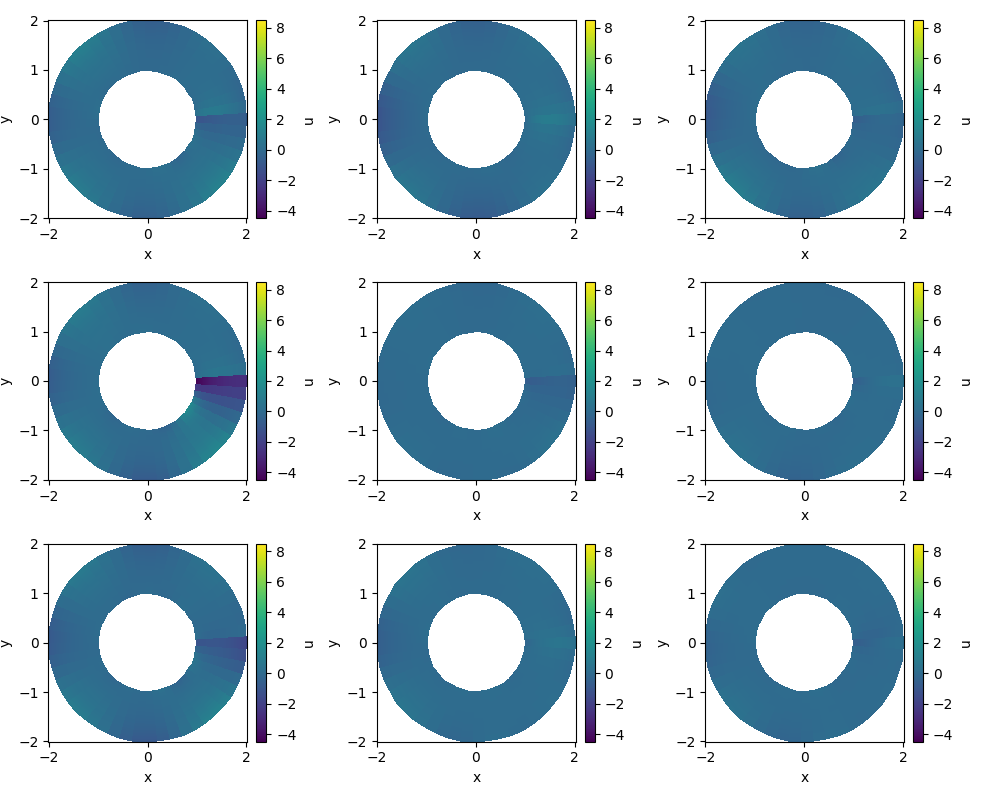
\includegraphics[width=\textwidth]{../plots/termal/solut dif l = (20x4) Nf=[1000, 5000, 10000] Nu=[100, 500, 1000].png}
    \caption{разница между аналитическим решением и решением нейросети при различных $N_f$ и $N_u$}
    \label{fig:termal_dif}
\end{figure}

\FloatBarrier
\newpage
\section{Заключение}

Мы написали, обучили и протестировали PINN, который решает задачу распределения тепла в кольце. Нам удалось получить в целом достаточно хорошее решение, близкое к истинному, однако решение занимает относительно много времени, что делает нецелесообразным использование PINN в текущем варианте. Так же нами были высказаны предположения по улучшению точности решения и ускорению работы PINN.
\newpage

\bibliographystyle{unsrt}
\bibliography{otchet}

\end{document}